\documentclass[12pt]{article}

\usepackage{amsthm}
\usepackage{amsmath}
\usepackage{graphicx}
\graphicspath{ {images/}{plots/} }
\usepackage{listings}
\lstset{
  basicstyle=\ttfamily,
  columns=fullflexible,
  frame=single,
  breaklines=true,
}

\theoremstyle{definition}
\newtheorem{definition}{Definition}

\title{{\small{Machine Learning and Algorithms for Data Mining} \\
Assessment 1:} \\
\textit{Computing Communities in Large Networks Using Random Walks}}
\author{Sebastian Borgeaud --- spb61@cam.ac.uk}

\begin{document}
\maketitle

\begin{abstract}
	In this report, I first report the key ideas and concepts introduced in ``Computing Communities in Large Networks Using Random Walks'' \cite{pons2005computing}. Next, I present my Python implementation of the algorithm. Finally, I compare the results produced by my algorithm with those reported in \cite{pons2005computing} and evaluate my algorithms on multiple real world test networks.
	\end{abstract}

\section{Main contributions, Key Concepts and Ideas}
The paper presents a clustering method for large undirected graphs based on random walks. The paper is based upon the idea that before a random walk converges to the stationary distribution, it should spend more time travelling inside clusters than moving between clusters, for a suitable definition of clusters. In fact, we can use this to create clusters.

\subsection{Random walks on graphs}
More formally, consider an undirected graph $G=(V,E)$ where $V$ are the vertices and $E$ are the edges of $G$. Let $n = |V|$ and $m = |E|$. This graph has an \textbf{adjacency matrix} $A$, given by
\[ 
A_{i,j} = 
\begin{cases}
	1, 	&\textnormal{ if $(i,j) \in E$},\\
	0	&\textnormal{otherwise}\\
\end{cases}
\]

The paper makes two assumptions about the undirected graphs we work with:
\begin{enumerate}
	\item Every node in the graph is connected to itself.
	\item The graph is connected, that is we can reach any node from any starting node.
\end{enumerate}

We can define a random walk on this graph using the \textbf{transition matrix} $P$, given by:
\begin{equation}
	P_{i,j} = \frac{A_{i,j}}{d(i)}
\end{equation}
where $d(i) = \Sigma_j A_{i,j}$ denotes the \textbf{degree} of node $i$. This means that if at time $t$ the random walker is at node $i$, it will move with probability $P_{i,j}$ to node $j$, i.e.\ move to a neighbour with uniform probability.

\subsection{Distance between vertices and distance between clusters}
For a random walk of length $t$, the probability of starting at node $i$ and ending at node $j$ is given by $P_{i,j}^t$. If $t$ is large enough to gather some information about the structure of the graph, but not too large as to make $P_{i,j}^t$ converge to the stationary distribution, $P_{i,j}^t$ can be used to define a notion of distance between two nodes of the graph, as it has the following desirable properties:
\begin{enumerate}
	\item If two vertices $i$ and $j$ are in the same cluster, then $P_{i,j}^t$ should be high.
	\item The probability of $P_{i,j}^t$ is influenced by $d(j)$ as the walker is more likely to go to high degree vertices.
	\item A random walk starting from a vertex $i$ or $j$ of the same cluster, should end in vertex $k$ with similar probability. That is for every vertex $k$, $P_{i,k}^t$  and $P_{j,k}^t$ should be similar.
\end{enumerate}
We can now define the distance between two vertices $i$ and $j$:
\begin{definition}
	We can now define the distance between two vertices $i$ and $j$:
	\[ r_{i,j} = \sqrt{\sum_{k=1}^n \frac{(P_{i,k}^t - P_{j,k}^t)^2}{d(k)}} \]
\end{definition}
Note this is really an euclidian distance:
\[ r_{i,j} = \|D^{-\frac{1}{2}}P_{i,\bullet}^t - D^{-\frac{1}{2}}P_{j,\bullet}^t \|\]
where $D_{i,j} = \delta_{i,j} \cdot d(i)$ is the diagonal matrix of the degrees of the vertices in $G$ and $P_{i,\bullet}^t$ is the column vector containing probabilities $(P_{i,k}^t)_{1 \le k \le n}$.
Next, we can generalise this notion of distance to clusters.
\begin{definition}
	Let $C_1, C_2 \subset V$ be two clusters in $G$. The distance $r_{C_1,C_2}$ is defined to be:
	\[ r_{C_1,C_2} = \sqrt{\sum_{k=1}^n \frac{(P_{C_1,k}^t - P_{C_2,k}^t)^2}{d(k)}} \]
\end{definition}
where the probability $P_{C,k}^t$ to go from cluster $C$ to vertex $k$ in $t$ steps is defined to be
\[ P_{C,k}^t = \frac{1}{|C|}\sum_{i \in C}P_{i,k}^t\]
Again, this is really an euclidean distance as 
\[  r_{C_1,C_2} = \|D^{-\frac{1}{2}}P_{C_1,\bullet}^t - D^{-\frac{1}{2}}P_{C_2,\bullet}^t \|\]

\subsection{Clustering algorithm}
The distance introduced earlier can be used in a hierarchical clustering algorithm. First, we initialise the initial partition of the graph into $n$ clusters, one per vertex: $\mathcal{P}_1 = \{\{v\} \mid v \in V\}$. Then the algorithm repeatedly merges clusters until only a single cluster is left, by repeating at each step $k$:
\begin{enumerate}
	\item Choose two closest clusters $C_1$ and $C_2$ to merge.
	\item Merge $C_1$ and $C_2$.
	\item Update the distances between $C_3$ and its adjacent clusters.
	\item Create a new partition $\mathcal{P}_{k+1} = (\mathcal{P} \setminus \{C_1, C_2\}) \cup C_3$
\end{enumerate}
\subsubsection{Choosing two clusters to merge}
In order to reduce the complexity and to guarantee that every cluster is connected, that is any node in a cluster can be reached from every other node in the cluster without leaving the cluster, only adjacent clusters are considered for merging.

The two clusters are then chosen to be those that, when merged, minimise 
\[\sigma_k = \frac{1}{n} \sum_{C \in \mathcal{P}_k} \sum_{i \in C} r_{i,C}^2\]
This is usually a NP-hard problem. However, for our definition of $r_{i,C}$, we can compute the variation $\Delta\sigma(C_1,C_2)$ that would be induced by merging $C_1$ with $C_2$, where
\[\Delta\sigma(C_1,C_2) = \frac{1}{n} \big( \sum_{i \in C_3} r_{i,C_3}^2 - \sum_{i \in C_1} r_{i,C_1}^2 - \sum_{i \in C_2} r_{i,C_2}^2 \big)\]
One can show that $\Delta\sigma(C_1,C_2)$ is related to $r_{C_1, C_2}$ by:
\begin{equation}
	\label{eq_theorem3}
	\Delta\sigma(C_1,C_2) = \frac{1}{n}\frac{|C_1||C_2|}{|C_1| + |C_2|} r_{C_1,C_2}^2 
\end{equation}
which allows for a more efficient computation.
\subsubsection{Merging the clusters}
This step is straightforward as the new cluster $C_3$ consists of the nodes in $C_1$ and $C_2$:
\[ C_3 = C_1 \cup C_2 \]
The updated probability vector $P_{C_3,\bullet}^t$ is computed using $P_{C_1,\bullet}^t$ and $P_{C_2,\bullet}^t$:
\begin{equation}
\label{eq_update_P_t}
P_{C_3,\bullet}^t = \frac{C_1 P_{C_1,\bullet}^t + |C_2| P_{C_2,\bullet}^t}{|C_1| + |C_2|}
\end{equation}

\subsubsection{Updating the distances}
Next, we need to compute the updated variation $\Delta\sigma(C_3, C)$ for every other cluster C. There are two cases to consider:
\begin{enumerate}
	\item If $C$ is adjacent to both $C_1$ and $C_2$, then we already have the values of $\Delta\sigma(C_1, C)$ and $\Delta\sigma(C_2, C)$. It is then possible to compute $\Delta\sigma(C_3, C)$ in constant time using:
	\begin{equation}
	\label{eq_theorem4}
	\Delta\sigma(C_3, C) = \frac{(|C_1| + |C|) \Delta\sigma(C_1,C) + (|C_2| + |C|) \Delta\sigma(C_2,C) + |C| \Delta\sigma(C_1,C_2)}{|C_1| + |C_1| + |C|}
	\end{equation}
	\item If $C$ is adjacent to only $C_1$ or $C_2$, we have to compute $\Delta\sigma(C_3, C)$ using equation \ref{eq_theorem3}, that is
	\begin{equation}
	\label{eq_theorem3}
	\Delta\sigma(C_3,C) = \frac{1}{n}\frac{|C_3||C|}{|C_3| + |C|} r_{C_3,C}^2 
	\end{equation}
\end{enumerate}

\subsection{Evaluating the partitions}
The final step of the algorithm is to choose the partition $\mathcal{P}_k$ that best captures the notion of community for our graph. The paper presents two methods for this:
\begin{enumerate}
	\item Choose the partition $\mathcal{P}$ that maximises the modularity $Q$, defined as
	\[ Q(\mathcal{P}) = \sum	_{C \in \mathcal{P}} e_C - a_C^2\] 
	where $e_C$ is the fraction of edges inside cluster $C$ and $a_C$ is the fraction of edges bound to cluster $C$.
	\item An alternative is to use the partition $\mathcal{P}$ associated with the largest value of the increase ratio
	\[ \eta_k = \frac{\Delta\sigma_k}{\Delta\sigma_{k-1}}\].
	This relies on the idea that if we merge two clusters that are very different in step $k$, then $\Delta\sigma_k$ will be large and thus, if $\Delta\sigma_k$ is large, then the clusters at step $k-1$ must be relevant.
\end{enumerate}

%\subsection{Complexity}

\section{Implementation}
I implemented this algorithm in Python, making use of \texttt{numpy} to handle the computations over the matrices and vectors.

\subsection{Initialisation of $P^t$}
The first step is to compute the probability vectors $P_{i,\bullet}^t$ from the adjacency matrix $A$. This can be done efficiently with numpy as 
\[ P^t = P \cdot P^{t-1} \]
starting with $P^0=I$, where $I$ is the identity matrix. In python, using numpy we have:
\begin{lstlisting}[language=Python]
P_t = np.eye(N)
for i in range(t):
    P_t = np.dot(P, P_t)
\end{lstlisting}
The vector $P_{i,\bullet}^t$, then simply corresponds to the i\textsuperscript{th} row of the matrix \texttt{P\_t}.

\subsection{Initialisation of the clusters}
The second step is to initialise the clusters. For each cluster $C$, we need to keep the following information:
\begin{itemize}
	\item The nodes contained in the cluster
	\item The probability vector $P_{C,\bullet}^t$
	\item The neighbouring clusters
\end{itemize}
Furthermore, to keep the hierarchical algorithm simple, I keep for each neighbour cluster $C'$ of $C$, the variation $\Delta\sigma(C,C')$. This is slightly inefficient as we have duplicate information as $\Delta\sigma(C,C') = \Delta\sigma(C',C)$, but allows for a simpler implementation of the algorithm.

\bigskip

The clusters are therefore stored in a dictionary, \texttt{clusters}, with cluster $C_i$ at \texttt{clusters[i]}. Each cluster $C_i$ is itself a dictionary, where
\begin{itemize}
	\item \texttt{clusters[i]['nodes']} contains a Python set of the nodes in $C_i$.
	\item \texttt{clusters[i]['P\_t']} contains a numpy vector representing $P_{C_i,\bullet}^t$.
	\item \texttt{clusters[i]['neighbours']} contains a dictionary mapping every neighbouring cluster $C_j$ to $\Delta\sigma(C_i,C_j)$
\end{itemize}

\subsection{Hierarchical clustering}
The hierarchical clustering algorithm is implemented using two helper functions. 
\subsubsection{Finding two clusters $C_i$ and $C_j$ to merge}
The first one takes the dictionary of the current clusters in the partition and returns the ids of the two clusters $C_i$ and $C_j$ to merge in this step together with $\Delta\sigma(C_i,C_j)$. 

This step is straightforward using an $\mathcal{O}(M)$ implementation where $M$ is the number of edges in the graph. I simply iterate over all pairs of neighbouring clusters and find the two clusters whose variation is the smallest. The python implementation is
\begin{lstlisting}[language=Python, mathescape]
def find_to_merge(clusters):
    min_$\Delta\sigma$ = None
    to_merge = None
    for i, cluster in clusters.items():
        for j, dist in cluster['neighbours'].items():
            if min_$\Delta\sigma$ == None or dist < min_$\Delta\sigma$:
                min_$\Delta\sigma$ = dist
                to_merge = (i, j)
    return (to_merge[0], to_merge[1], min_$\Delta\sigma$)
\end{lstlisting}


\subsubsection{Merging two clusters $C_i$ and $C_j$}
The second helper function takes in the ids of two clusters to merge and a fresh identity \texttt{new\_id} and updates the dictionary \texttt{clusters} by merging the two clusters into a new cluster, associating the new cluster with \texttt{new\_id}.

This helper function needs to create a new cluster \texttt{C3} from the two cluster \texttt{C1} and \texttt{C2}. First, we can create the set of nodes in \texttt{C3} as it is simply the union of the set of nodes in \texttt{C1} and \texttt{C2}.

Next, we compute the new probability vector $P_{\texttt{C3}, \bullet}^t$ using equation \ref{eq_update_P_t}.

Finally, we update the variations $\Delta\sigma(\texttt{C3}, \texttt{C})$ for every cluster \texttt{C} now adjacent to \texttt{C3}. To do this we first compute the set of new neighbours of \texttt{C3}, \texttt{new\_neighbours}. This set consists of all clusters \texttt{C} that were adjacent to \texttt{C1} or adjacent to \texttt{C2}. Then we compute $\Delta\sigma(\texttt{C3}, \texttt{C})$ using either equation \ref{eq_theorem4} or equation \ref{eq_theorem3} depending on whether \texttt{C} was adjacent to both \texttt{C1} and \texttt{C2}, or to only one of the two clusters. Note that we also need to update the dictionary of neighbours for cluster \texttt{C} by removing the entries for \texttt{C1} and \texttt{C2}, and addding a new entry for \texttt{C3}. 

The full implementation of this function is:
\begin{lstlisting}[language=Python, mathescape]
def merge_clusters(clusters, i, j, new_id):
    C1 = clusters[i]
    C2 = clusters[j]    
    l1 = len(C1['nodes'])
    l2 = len(C2['nodes'])
    
    C3 = {}
    C3['nodes'] = C1['nodes'].union(C2['nodes'])
    C3['P_t'] = (l1 * C1['P_t'] + l2 * C2['P_t']) / (l1 + l2)

    new_neighbours = set(C1['neighbours'].keys()).union(set(C2['neighbours'].keys()))
    new_neighbours.remove(i)
    new_neighbours.remove(j)
    
    C3['neighbours'] = {}
    for n in new_neighbours:
        C = clusters[n]
        l3 = len(C['nodes'])
        if n in C1['neighbours'].keys() and n in C2['neighbours'].keys():
            x_A = (l1 + l3) * C1['neighbours'][n]
            x_B = (l2 + l3) * C2['neighbours'][n]
            x_C = (l3) * C1['neighbours'][j]
            new_$\Delta\sigma$ = (x_A + x_B - x_C) / (l1 + l2 + l3)
        else:
            new_$\Delta\sigma$ = $\Delta\sigma$(l1+l2, C3['P_t'], l3, C['P_t'])
        
        C3['neighbours'][n] = new_$\Delta\sigma$
        C['neighbours'].pop(i, None)
        C['neighbours'].pop(j, None)
        C['neighbours'][new_id] = new_$\Delta\sigma$
    
    clusters[new_id] = C3
    clusters.pop(i)
    clusters.pop(j)
\end{lstlisting}
    
\subsubsection{Hierarchical clustering algorithm}
Using the two helper functions as stated above, the main loop of the algorithm becomes very simple, repeatedly finding two clusters to merge and then merging them:
\begin{lstlisting}[language=Python, mathescape]
new_id = N #next cluster starts with id N

while(len(clusters) > 1):    
    # find clusters to merge
    (i,j, min_$\Delta\sigma$) = find_to_merge(clusters)
    # Compute new partion
    merge_clusters(clusters, i, j, new_id)
    # increment id for next cluster
    new_id += 1
\end{lstlisting}
However, as we need to be able to rebuild the dendogram, to compute the modularity and to compute the increase ratio at each step, we need to keep some additional information at each step $k$. First, to be able to later reconstruct the dendogram, at each time step I append the tuple \texttt{(new\_id, i, j, cum\_dist)}  to a list \texttt{build\_tree}, representing the fact that clusters with ids \texttt{i} and \texttt{j} have been merged into a cluster with id \texttt{new\_id}. The value \texttt{cum\_dist} represent the cumulative variation that has occurred since up to this merging, i.e.\ $\texttt{cum\_dist} = \sum_{i=1}^k \texttt{min\_}\Delta\sigma_k$.

Next, the partition $\{C \mid C \in \texttt{clusters[i]['nodes']} \}$ is append to a list named \texttt{partitions} representing $\mathcal{P}$.

Finally, to be able to compute the increase ration $\eta_k$, I keep the minimum variation \texttt{min\_$\Delta\sigma$} in a list \texttt{$\Delta\sigma$s}.

The full version of the main loop is therefore:
\begin{lstlisting}[language=Python, mathescape]
new_id = N
build_tree = []
$\Delta\sigma$s = []
partitions = [create_partition(clusters)]
cum_dist = 0

while(len(clusters) > 1):    
    # find clusters to merge
    (i,j, min_$\Delta\sigma$) = find_to_merge(clusters)
    # Compute new partion
    merge_clusters(clusters, i, j, new_id)
    
    # For rebuilding the dendogram
    build_tree.append((new_id, i, j, cum_dist))
    cum_dist += min_$\Delta\sigma$
    
    # Keep track of partitions
    partitions.append(create_partition(clusters))
    
    # For evaluation of partitions
    Δσs.append(min_$\Delta\sigma$)
    
    new_id += 1	
\end{lstlisting}

\section{Results \& analysis}


\subsection{Example graph from the paper}
To check that my implementation matches the one given in the paper, I reuse the simple toy network consisting of 16 nodes (see figure \ref{fig_toy_graph}) given on page 11 of the paper.
\begin{figure}
	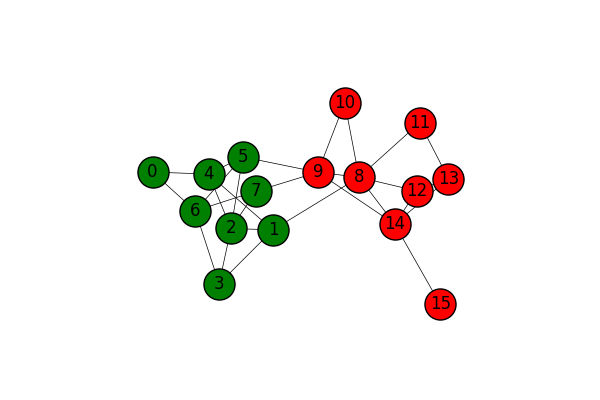
\includegraphics[scale=0.6]{toy_graph}
	\centering
	\caption{Simple graph with 16 vertices given in the paper on page 11.}
	\label{fig_toy_graph}
\end{figure}
Running my implementation on this graph gives the dendogram shown in figure \ref{fig_toy_graph_dendogram}. As expected, this is the same dendogram as the one given in the paper. Furthermore, the increase ratios and the modularities for each  partition $\mathcal{P}_k$, see figure \ref{fig_toy_graph_eval}, also match the values given in the paper.

\begin{figure}
	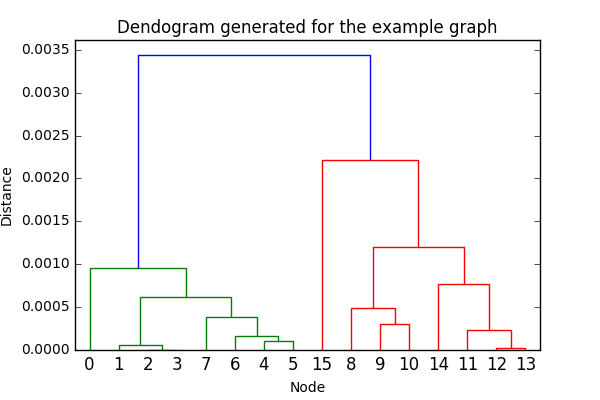
\includegraphics[scale=0.5]{toy_graph_dendogram}
	\centering
	\caption{Dendogram resulting from runnign my implementation of the clustering algorithm on the simple toy graph. The resulting dendogram matches the one given in the paper.}
	\label{fig_toy_graph_dendogram}
\end{figure}
\begin{figure}
	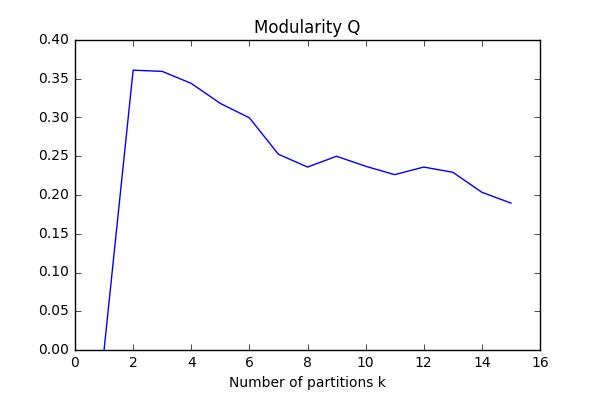
\includegraphics[scale=0.44]{toy_graph_Q}
	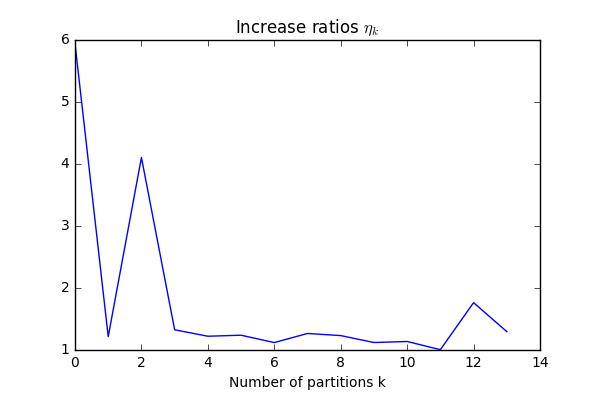
\includegraphics[scale=0.44]{toy_graph_eta}
	\centering
	\caption{Modularity and increase ratios for the toy example graph given in the paper. The curves match those given in the paper.}
	\label{fig_toy_graph_eval}
\end{figure}

%\begin{figure}
%	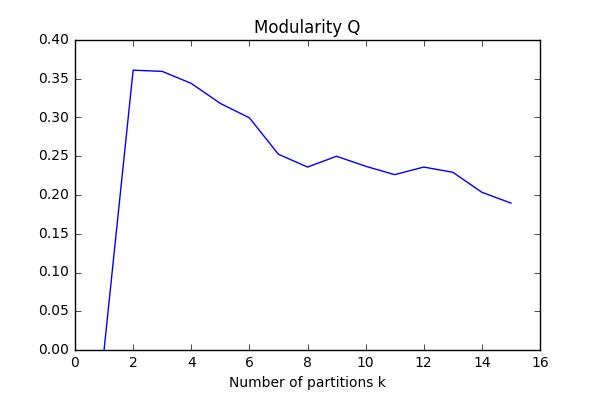
\includegraphics[scale=0.44]{toy_graph_Q}
%	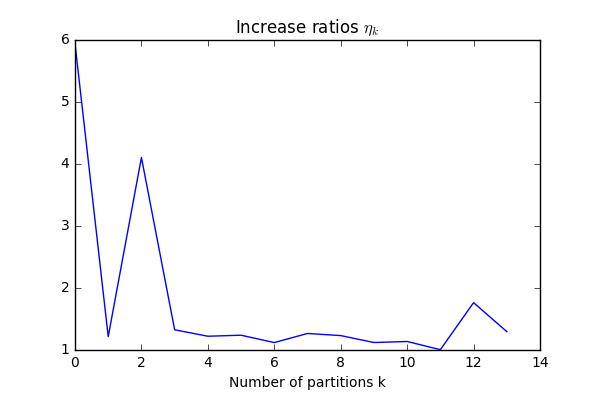
\includegraphics[scale=0.44]{toy_graph_eta}
%	\centering
%	\caption{Modularity and increase ratios for the toy example graph given in the paper. The curves match those given in the paper.}
%	\label{fig_toy_graph_eval}
%\end{figure}

Finally, using the partition into two clusters as suggested by both the modularity and the increase ratios, we can recover the same partition as the one given in the paper, i.e.\ the partition into the two clusters denoted by green and red nodes in figure \ref{fig_toy_graph}.

\subsection{Test on randomly generated graph}
Testing a graph clustering algorithm is a hard task as we need to evaluate the resulting partition. A common way to do this is to use randomly generated graphs for which the partition is already known.

\subsection{Zachary's karate club \cite{zachary1977information}}
The next graph I use to test my implementation of the algorithm is the Zachary's karate club network, drawn in figure \ref{fig_karate_graph}. The graph represents the friendship of the 34 members of a karate club. The club then split into two groups as a result of a dispute, the members of each group starting their own club. The question we can now ask is if our algorithm is able to recover these two groups.
\begin{figure}[h]
	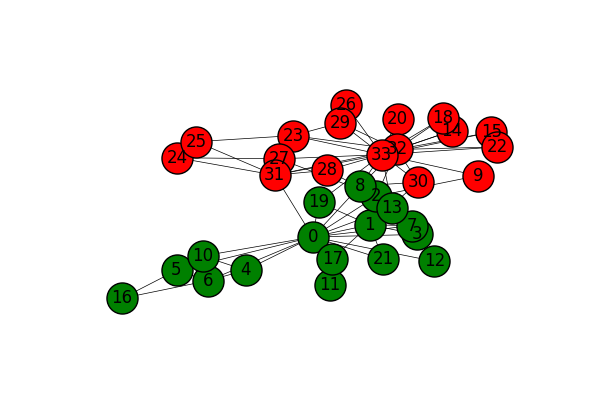
\includegraphics[scale=0.5]{karate_graph}
	\centering
	\caption{Zachary's karate club network.}
	\label{fig_karate_graph}
\end{figure}
Running the algorithm on this graphs, gives the dendogram given in figure \ref{fig_karate_graph_dendogram}.
\begin{figure}
	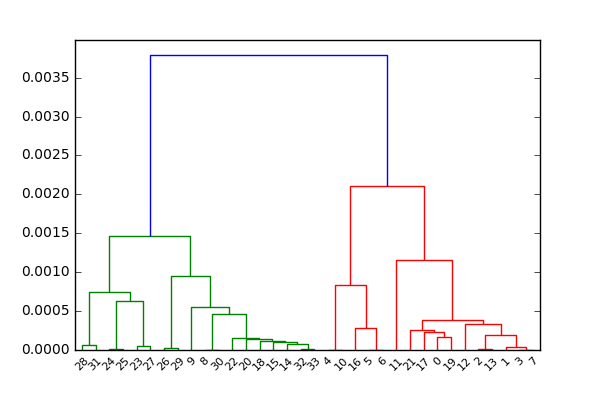
\includegraphics[scale=0.5]{karate_dendogram}
	\centering
	\caption{Dendogram resulting from using our algorithm on Zachary's karate club network.}
	\label{fig_karate_graph_dendogram}
\end{figure}

Analysing the partitions using modularity and the increase ratio (figure \ref{fig_karate_eval}), we can see that the algorithm suggests a partition into either 2 or 4 clusters. These partitions are shown in figure \ref{fig_toy_graph_partitions}. For the partition into two clusters every node has been assigned the correct cluster except for node 8.

\begin{figure}
	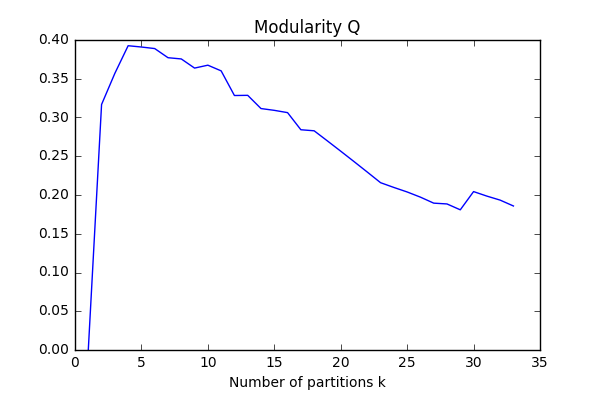
\includegraphics[scale=0.44]{karate_graph_Q}
	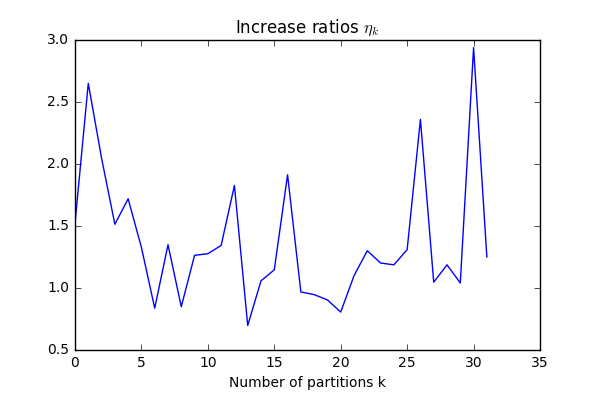
\includegraphics[scale=0.44]{karate_graph_eta}
	\centering
	\caption{Modularity and increase ratios for the Karate Club network. The modularity suggests a partition into 4 clusters. The increase ration suggests a partition into 2 clusters, as we can disregard clustering the network into more than 10 clusters.}
	\label{fig_karate_eval}
\end{figure}
\begin{figure}
	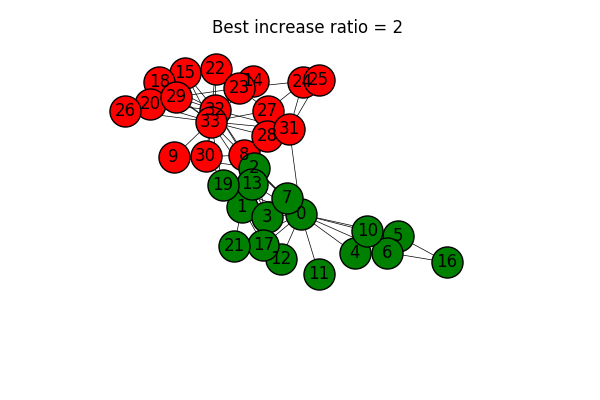
\includegraphics[scale=0.44]{karate_graph_partition2}
	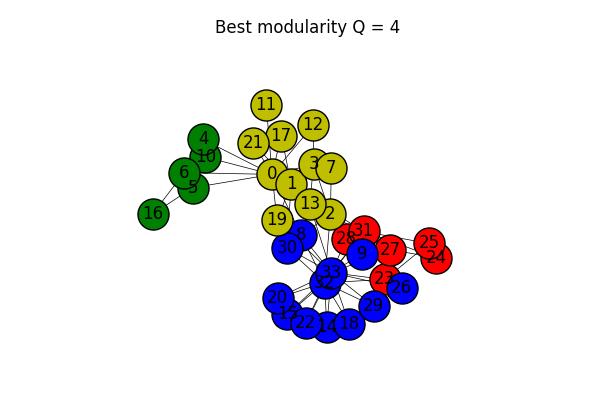
\includegraphics[scale=0.44]{karate_graph_partition4}
	\centering
	\caption{Partition into 2 and 4 clusters given by our algorithm for the Zachary's karate club network. For the partition into 2 clusters, every node has been assigned the correct cluster, except node 8.}
	\label{fig_toy_graph_partitions}
\end{figure}

\subsection{American college football \cite{girvan2002community}}
Next, I test the algorithm on the American College Football network \cite{girvan2002community}. The graph consists of 155 nodes, each node being assigned into one of 12 conferences. The question to ask is whether my implementation of the algorithm can recover this partitioning into the 12 conferences. The modularities and the increase ratios obtained are shown in figure \ref{fig_football_eval}.
\begin{figure}
	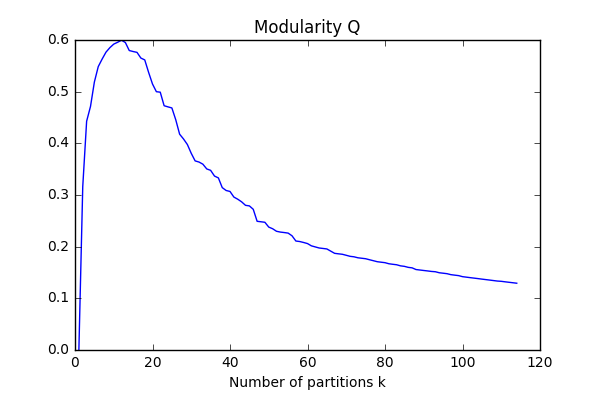
\includegraphics[scale=0.44]{football_graph_Q}
	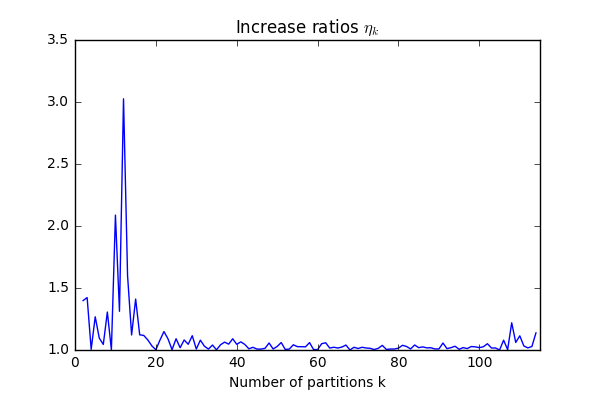
\includegraphics[scale=0.44]{football_graph_eta}
	\centering
	\caption{Modularity and increase ratios for the American College Football network. The modularity is maximised at a partition into 12 clusters, with a value of 0.6. The increase ration suggests a partition into 10 clusters.}
	\label{fig_football_eval}
\end{figure}
The modularity is maximised at a partition into 12 clusters, with a value of 0.6. Indeed, using the generated partition for 12 clusters, the algorithm is able to approximately recover the 12 conferences, with only 10 nodes being misclassified. 

\bibliography{bib}
\bibliographystyle{unsrt}


\end{document}